\documentclass[11pt,a4paper]{report}

\usepackage{amssymb,amsmath,epsfig,float,subfig,hyperref,multicol}
\usepackage{morefloats,graphicx}

\usepackage{xcolor}

\definecolor{SCSUred}{HTML}{CD1041}

\hypersetup{colorlinks=true,linkcolor=SCSUred,urlcolor=SCSUred}

\usepackage{enumerate}
\usepackage{tikz}
\usetikzlibrary{arrows}
\usetikzlibrary{patterns}
\usetikzlibrary{decorations}
%%\usetikzlibrary{intersections}
\usetikzlibrary{matrix}
\usetikzlibrary{snakes}
\usetikzlibrary{calc}
\usetikzlibrary{backgrounds}

\definecolor{linecolor}{HTML}{0074C8}
\definecolor{linecolor2}{HTML}{C80200}

\newcommand{\imagebullet}[1]{\includegraphics[width=0.5cm]{#1}}

\pagestyle{empty}
\setlength{\textwidth}{7in}
\setlength{\textheight}{10in}
\setlength{\oddsidemargin}{-25pt}
\setlength{\evensidemargin}{-25pt}
\setlength{\topmargin}{-50pt}

\usepackage[english]{babel}
\usepackage[utf8]{inputenc}
\usepackage{fancyhdr}
 
%%\pagestyle{fancy}
\renewcommand{\headrulewidth}{0pt}
%%\fancyhf{}
%%\rhead{Share\LaTeX}
%%\lhead{Guides and tutorials}
%%\cfoot{OVER}

\newcommand{\DueA}{Tuesday, November 12}
\newcommand{\DueB}{Thursday, November 14}
\newcommand{\DueC}{Monday, November 25}

\begin{document}

\begin{figure}[ht]
\begin{flushright}
	\includegraphics[width=2.0in]{U_PriHorz_WhtLtBG.jpg}
	\end{flushright}
\end{figure}

\vspace{-12mm}

\begin{flushleft}
\Large\bf \href{https://activecalculus.org/single/sec-4-3-definite-integral.html}{4.3 - The Definite Integral}\rm
%%Daily Preparation - \DueA \rm
\end{flushleft}


\vspace{8pt}

\noindent {\Large\bf{Overview}} \\
In this section we introduce a notation used for expressing the limit of a Riemann sum. We thus define what a definite integral is. We will be discussing the definition, meaning, and use of the definite integral for the remainder of the course. Surprisingly, it has a very strong and natural connection to the derivative -- a connection we will discuss and explore in Section 4.4. However, in this section, we deduce the properties that this new mathematical object, the definite integral, has based on its definition and its geometrical interpretation.



\vspace{16pt}

%%\pagebreak

\noindent {\Large\bf{To prepare for class}} \\
Complete all actions listed below.  Respond to the questions highlighted with {\color{SCSUred}{\boxed{Submit}}}.  %% by the start of class on {\bf{\DueA}}.  A single .pdf should be uploaded to D2L Brightspace.
\begin{itemize} \itemsep -2pt % Reduce space between items


\item {\bf{Read}} motivating questions and the introduction to \href{https://activecalculus.org/single/sec-4-3-definite-integral.html}{section 4.3} (up until Preview Activity 4.3.1).

\item[{\color{SCSUred} \boxed{Submit}}] {\bf{Do}} \href{https://activecalculus.org/single/sec-4-3-definite-integral.html#XLD}{Preview Activity 4.3.1}.  

\item {\bf{Watch}} video \href{https://www.youtube.com/watch?v=Lp5KsXN4UOQ&feature=emb_title}{Quick Review - The Definite Integral (3:00)}.   

\item {\bf{Read}} \href{https://activecalculus.org/single/sec-4-3-definite-integral.html#uqj}{section 4.3.1} up to Activity 4.3.2.  



\item[{\color{SCSUred} \boxed{Submit}}] {\bf{Explore}} the applet \href{http://webspace.ship.edu/msrenault/GeoGebraCalculus/integration_intro_geometric.html}{Gaining Geometric Intuition}.  Submit answers to questions \#3-6 at the bottom of the webpage.  

\item[\imagebullet{CopilotLogo.jpg}] Prompt {\bf{Copilot}} ``Please produce and execute Python code that illustrates an upper Riemann sum of the function $f(x)=\cos(x)+1$ from $x=0$ to $x=3\pi$ using n=10 rectangles."  

\item {\bf{Do}} these problems.
\begin{enumerate}
\setcounter{enumi}{0}

\item 
\begin{enumerate}
\item Use geometry to evaluate $\displaystyle \int_{-1}^4 1-\frac{1}{2}x \ dx$. 

\vspace{-20mm}
\begin{figure}[H]
\flushright
{
  \begin{tikzpicture}[thick,scale=1] 
%%\draw[step=1cm,color=gray!50,dotted] (0,-3) grid (5,3);
   \draw [black!80,line width=0.3pt,-latex] (0,0) -- (5,0) node [below] at (4.75,0) {$x$};
   \draw [black!80,line width=0.3pt,-latex] (0,0) -- (-1.5,0);
   \draw [black!80,line width=0.3pt,-latex] (0,0) -- (0,3) node [right] at (0,2.75) {$y$};
   \draw [black!80,line width=0.3pt,-latex] (0,0) -- (0,-1.5);
\draw[color=linecolor, line width=1pt,domain=-1:4]   plot (\x,{1-0.5*\x}) node [right] at (1,1) {$y=1-\frac{1}{2}x$};

\foreach \x/\xtext in { -1/-1, 1/1, 2/2, 3/3, 4/4}
    \draw[shift={(\x,0)}] (0pt,3pt) -- (0pt,-3pt) node[below] {$\xtext$};
\foreach \y/\ytext in {-1/-1, 1/1, 2/2}
    \draw[shift={(0,\y)}] (-2pt,0pt) -- (2pt,0pt) node[left] {$\ytext$};
\end{tikzpicture}}  
\end{figure}

\item Compute $\displaystyle \int_0^3 f(x) \ dx$ for the function $f$ graphed.  
\end{enumerate}

\vspace{-15mm}
\begin{figure}[H]
\flushright
{
  \begin{tikzpicture}[thick,scale=1]
%%\draw[step=1cm,color=gray!50,dotted] (0,-3) grid (5,3);
   \draw [black!80,line width=0.3pt,-latex] (0,0) -- (4,0) node [below] at (3.75,0) {$x$};
   \draw [black!80,line width=0.3pt,-latex] (0,0) -- (-0.5,0);
   \draw [black!80,line width=0.3pt,-latex] (0,0) -- (0,2) node [right] at (0,1.75) {$y$};
   \draw [black!80,line width=0.3pt,-latex] (0,0) -- (0,-0.5);
\draw[color=linecolor, line width=1pt,domain=0:2,smooth]   plot (\x,{sqrt(1-(\x-1)*(\x-1))});
\draw[color=linecolor, line width=1pt,domain=2:3,smooth]   plot (\x,{\x-2});
\foreach \x/\xtext in { 1/1, 2/2, 3/3}
    \draw[shift={(\x,0)}] (0pt,3pt) -- (0pt,-3pt) node[below] {$\xtext$};
\foreach \y/\ytext in {1/1}
    \draw[shift={(0,\y)}] (-2pt,0pt) -- (2pt,0pt) node[left] {$\ytext$};
\end{tikzpicture}}  
\end{figure}

\item Use the table to estimate $\displaystyle \int_0^{12} f(x) \ dx$.  Find a left sum $L_4$, a right sum $R_4$, and then average the two.  
\begin{center}
\begin{tabular}{l|c|c|c|c|c}
\hline
$x$ & 0 & 3 & 6 & 9 & 12\\
\hline
$f(x)$ & 20 & 10 & 5 & 2 & 1 \\
\hline
\end{tabular}
\end{center}

\pagebreak


\item[{\color{SCSUred} \boxed{Submit}} 3.] Each figure below illustrates a Riemann sum approximation, $\displaystyle \sum_{k=1}^n f(x_k^*) \Delta x_k$, to $\displaystyle \int_a^b f(x) \ dx$.  In each, determine the values of $a, b$, and $n$.  Then, give expressions for $\Delta x_k$ and $x_k^*$.  

\begin{figure}[H]
\centering
  \subfloat[ ][ ]
{
  \begin{tikzpicture}[thick,scale=1.25]
 
      \fill [linecolor!20] (1,0) -- (1,1.455) -- (2,1.455) -- (2,0) -- (1,0);
    \draw[black] (1,0) -- (1,1.455) -- (2,1.455) -- (2,0) -- (1,0);
          \fill [linecolor!20] (2,0) -- (2,1.067) -- (3,1.067) -- (3,0) -- (2,0);
    \draw[black] (2,0) -- (2,1.067) -- (3,1.067) -- (3,0) -- (2,0);
              \fill [linecolor!20] (3,0) -- (3,0.842) -- (4,0.842) -- (4,0) -- (3,0);
    \draw[black] (3,0) -- (3,0.842) -- (4,0.842) -- (4,0) -- (3,0);
%%\draw[step=1cm,color=gray!50,dotted] (0,-3) grid (5,3);
   \draw [black!80,line width=0.3pt,-latex] (0,0) -- (5,0) node [below] at (4.75,0) {$x$};
   \draw [black!80,line width=0.3pt,-latex] (0,0) -- (-0.5,0);
   \draw [black!80,line width=0.3pt,-latex] (0,0) -- (0,3) node [right] at (0,2.75) {$y$};
   \draw [black!80,line width=0.3pt,-latex] (0,0) -- (0,-0.5);
\draw[color=linecolor, line width=1pt,domain=1:4]   plot (\x,{4/(\x+1))}) node [above] at (1.5,2) {$\displaystyle f(x)$};
%%node [right] at (3,3) {$y=1-x^2$};
\foreach \x/\xtext in { 1/1, 2/2, 3/3, 4/4}
    \draw[shift={(\x,0)}] (0pt,3pt) -- (0pt,-3pt) node[below] {$\xtext$};
\foreach \x/\xtext in {0.25, 0.5, 0.75, 1, 1.25, 1.5, 1.75, 2, 2.25, 2.5, 2.75, 3, 3.25, 3.5, 3.75}
    \draw[shift={(\x,0)}] (0pt,1.5pt) -- (0pt,-1.5pt);
%% node[below] {$\xtext$};
\foreach \y/\ytext in {1/1, 2/2}
    \draw[shift={(0,\y)}] (-2pt,0pt) -- (2pt,0pt) node[left] {$\ytext$};
\end{tikzpicture}}  
\hspace{0.1in}            
 \subfloat[ ][ ]
{
  \begin{tikzpicture}[thick,scale=1.25]
       \fill [linecolor!20] (0.5,0) -- (0.5,2.667) -- (1,2.667) -- (1,0) -- (0.5,0);
    \draw[black] (0.5,0) -- (0.5,2.667) -- (1,2.667) -- (1,0) -- (0.5,0);
      \fill [linecolor!20] (1,0) -- (1,2) -- (1.5,2) -- (1.5,0) -- (1,0);
    \draw[black] (1,0) -- (1,2) -- (1.5,2) -- (1.5,0) -- (1,0);
          \fill [linecolor!20] (1.5,0) -- (1.5,1.6) -- (2,1.6) -- (2,0) -- (1.5,0);
    \draw[black] (1.5,0) -- (1.5,1.6) -- (2,1.6) -- (2,0) -- (1.5,0);
              \fill [linecolor!20] (2,0) -- (2,1.333) -- (2.5,1.333) -- (2.5,0) -- (2,0);
    \draw[black] (2,0) -- (2,1.333) -- (2.5,1.333) -- (2.5,0) -- (2,0);
                  \fill [linecolor!20] (2.5,0) -- (2.5,1.143) -- (3,1.143) -- (3,0) -- (2.5,0);
    \draw[black] (2.5,0) -- (2.5,1.143) -- (3,1.143) -- (3,0) -- (2.5,0);
                      \fill [linecolor!20] (3,0) -- (3,1) -- (3.5,1) -- (3.5,0) -- (3,0);
    \draw[black] (3,0) -- (3,1) -- (3.5,1) -- (3.5,0) -- (3,0);
%%\draw[step=1cm,color=gray!50,dotted] (0,-3) grid (5,3);
   \draw [black!80,line width=0.3pt,-latex] (0,0) -- (5,0) node [below] at (4.75,0) {$x$};
   \draw [black!80,line width=0.3pt,-latex] (0,0) -- (-0.5,0);
   \draw [black!80,line width=0.3pt,-latex] (0,0) -- (0,3) node [right] at (0,2.75) {$y$};
   \draw [black!80,line width=0.3pt,-latex] (0,0) -- (0,-0.5);
\draw[color=linecolor, line width=1pt,domain=0.5:3.5]   plot (\x,{4/(\x+1))}) node [above] at (1.5,2) {$\displaystyle f(x)$};
%%node [right] at (3,3) {$y=1-x^2$};

\foreach \x/\xtext in { 1/1, 2/2, 3/3, 4/4}
    \draw[shift={(\x,0)}] (0pt,3pt) -- (0pt,-3pt) node[below] {$\xtext$};
\foreach \x/\xtext in {0.25, 0.5, 0.75, 1, 1.25, 1.5, 1.75, 2, 2.25, 2.5, 2.75, 3, 3.25, 3.5, 3.75}
    \draw[shift={(\x,0)}] (0pt,1.5pt) -- (0pt,-1.5pt);
%% node[below] {$\xtext$};
\foreach \y/\ytext in {1/1, 2/2}
    \draw[shift={(0,\y)}] (-2pt,0pt) -- (2pt,0pt) node[left] {$\ytext$};
\end{tikzpicture}}  
\end{figure}





\end{enumerate}




\item[\imagebullet{CopilotLogo.jpg}] Prompt {\bf{Copilot}} ``Please produce and execute Python code that illustrates a middle Riemann sum of the function f(x)=x$\wedge$2+1 from x=1 to x=3 using n=5 rectangles."  Does the AI give you a correct value for the sum being illustrated?


\item {\bf{Read}} \href{https://activecalculus.org/single/sec-4-3-definite-integral.html#axs}{section 4.3.2} on properties of the definite integral. 

\item {\bf{Watch}} video \href{https://www.youtube.com/watch?v=1SqpYAAyBCk&feature=emb_title}{Evaluating Definite Integrals using Integral Properties (8:14)}. 

\item {\bf{Do}} this problem.
\begin{enumerate}
\setcounter{enumi}{3}

\item Suppose $f(x)$ is an odd function (as shown) with $\displaystyle \int_{-2}^0 f(x) \ dx = 4$.  \begin{enumerate}
\item Evaluate $\displaystyle \int_0^2 f(x) \ dx$ 

\item Evaluate $\displaystyle \int_{-2}^2 f(x) \ dx$

\item Evaluate $\displaystyle \int_{-2}^2 |f(x)| \ dx$ 

\end{enumerate} 

\vspace{-40mm}
\begin{figure}[H]
\begin{flushright}
	\includegraphics[width=2.5in]{fig_05_37.jpg}
	\end{flushright}
\end{figure}

\end{enumerate}

  
%%\item (Optional) {\bf{Do}} \href{https://activecalculus.org/single/sec-4-1-velocity-distance.html#gon}{Activity 4.1.2}. 

%%\item {\bf{Read}} \href{https://activecalculus.org/single/sec-4-1-velocity-distance.html#ldB}{section 4.1.2}.     

%%\item {\bf{Watch}} video \href{https://www.youtube.com/watch?v=mAul5vTAJSA&feature=emb_title}{Finding Distance Travelled with Antiderivatives (8:21)}.  


%%\item {\bf{Do}} \href{https://activecalculus.org/single/sec-4-1-velocity-distance.html#Ujq}{WebWork exercises 1-3 in section 4.1}. 



\end{itemize}













\vspace{16pt}

\noindent {\Large\bf{After class}}\\
Solidifying the concepts discussed in class through practice is necessary to build your skills. 

%%\noindent {\large\bf{After \DueA}}
\begin{itemize}\itemsep -2pt % Reduce space between items



\item {\bf{Read}} \href{https://activecalculus.org/single/sec-4-3-definite-integral.html#GEB}{section 4.3.3}.

\item {\bf{Watch}} video \href{https://www.youtube.com/watch?v=MQG9Nur4fdM&list=PL9bIjQJDwfGuXQHuS5Jkmum_CFILoCZX-&index=87}{Average Value of a Function (7:34)}.  
  

\item {\bf{Explore}} a nice visualization of \href{https://www.geogebra.org/m/m7GGErDY}{The Average Value of a Function}. 

  

\item {\bf{Explore}} \href{https://www.geogebra.org/m/nb34Cfvd}{the Average Value of a Linear Function} geometrically.  





%%\item {\bf{Do}} \href{https://activecalculus.org/single/sec-4-3-definite-integral.html#KUR}{Activity 4.3.4}.  
%%Solutions to this can be found here: \href{https://www.youtube.com/watch?v=iIjiyvV0Ma4}{Activity 4.2.4 video (6:27)}.  

\item {\bf{Do}} \href{https://activecalculus.org/single/sec-4-3-definite-integral.html#oxT}{exercises 1-2 in section 4.3}. 

\item {\bf{Do}} \href{https://activecalculus.org/single/sec-4-3-definite-integral.html#ZoV}{exercises 7-8 in section 4.3}.



%%\end{itemize}

%%\noindent {\large\bf{After \DueB}}
%%\begin{itemize}\itemsep -2pt % Reduce space between items

%%\item {\bf{Finish (if needed)}} \href{https://activecalculus.org/single/sec-4-3-definite-integral.html#BWE}{Activity 4.3.3}. 

\item {\bf{Read}} \href{https://activecalculus.org/single/sec-4-3-definite-integral.html#mLK}{section 4.3.4 - summary}.

\item {\bf{Do}} \href{https://activecalculus.org/single/sec-4-3-definite-integral.html#AMl}{(interactive) exercises 3-6 in section 4.3}. 

\item {\bf{Do}} \href{https://activecalculus.org/single/sec-4-3-definite-integral.html#lDn}{exercises 9-10 in section 4.3}.

%%\item {\bf{Do}} the following problem.
%%\begin{enumerate}
%%\setcounter{enumi}{4}

%%\item 


%%\end{enumerate}


\item {\bf{Start working}} on the \href{https://www.myopenmath.com/index.php}{MOMwork} (MyOpenMath) assignment for this section.  %%This will be due on \DueC. 

\end{itemize}

%%\pagebreak

\vspace{16pt}

\noindent {\Huge\bf{Extra Prep}}

\vspace{16pt}

\noindent {\Large\bf{Basic learning objectives}}\\
These are the tasks you should be able to perform with reasonable
fluency when you arrive at our next class meeting. Important new
vocabulary words are indicated {\it{in italics}}.  Check each box when you feel confident you have a firm grasp on that objective. 

\begin{itemize} \itemsep -2pt % Reduce space between items
\renewcommand{\labelitemi}{\scriptsize$\square$}
\item Recognize the parts of the limit definition of the definite integral, especially how the definite integral results from taking a limit of Riemann sums.

\item Identify an {\it{integral sign}}, {\it{integrand}}, and {\it{limits of integration}}.

\item Explain what it means to evaluate a {\it{definite integral}}.

\item Interpret, geometrically, the quantity denoted by $\displaystyle \int_a^b f(x) \ dx$. 

\item Recognize and apply properties that the definite integral possesses.  Use these properties to evaluate definite integrals in special circumstances.
\end{itemize}

\vspace{16pt}

\noindent {\Large\bf{Advanced learning objectives}}\\
In addition to mastering the basic objectives, here are the tasks you should be able to perform after class, with practice:
\begin{itemize} \itemsep -2pt % Reduce space between items
\renewcommand{\labelitemi}{\scriptsize$\square$}
\item Compute the {\it{average value of a function}} on the interval $[a,b]$ using $\displaystyle \int_a^b f(x) \ dx$.
\item Interpret the average value of a function as the height of a rectangle.
\end{itemize}

\vspace{16pt}

\noindent {\Large\bf{Need More Help?}}

\begin{itemize}\itemsep -2pt % Reduce space between items

\item {\bf{Watch}} video \href{https://www.youtube.com/watch?v=Dxmh7HMS2JM&feature=youtu.be}{Riemann Sum Notation (2:04)}.  

\item  {\bf{Watch}} video \href{https://www.youtube.com/watch?v=R6LQa_F-AFc&feature=youtu.be}{Riemann Sums - How to use Sigma Notation (6:33)}. 

\item {\bf{Finish (if needed)}} \href{https://activecalculus.org/single/sec-4-3-definite-integral.html#gJZ}{Activity 4.3.2}.
\begin{itemize}
\item (Optional) {\bf{Watch}} video \href{https://www.youtube.com/watch?v=F8lRiblAgD8}{explaining parts (a)-(c) of Activity 4.3.2 (4:00)}.  
\item (Optional) {\bf{Watch}} video \href{https://www.youtube.com/watch?v=bdDS594GSL0}{explaining part (d) of Activity 4.3.2 (2:47)}. 
\end{itemize}

\item  {\bf{Watch}} video \href{https://www.youtube.com/watch?v=5SIBNRXACWo&list=PLcJe72hRUmg7YrZ4OUkneU5jmyK4SEH9M&index=43}{Average Value of a Function with an Integral (2:09)}. 

\item  {\bf{Explore}} another way to visualize the \href{https://www.geogebra.org/m/UkTRUdU5}{Average Value of a Function}. 

\item  {\bf{Explore}} \href{https://www.geogebra.org/m/aXNuQYsp}{three more applets} illustrating the average value of a function.  

\item {\bf{Do}} these problems.
\begin{enumerate}
\setcounter{enumi}{4}

\item Consider approximating the definite integral $\displaystyle \int_{0.5}^5 \frac{4}{1+x} \ dx$ by a Riemann sum approximation $$ \sum_{k=1}^3 \frac{4}{1+\left[ 0.5+k \cdot \left( \frac{3}{2} \right)\right]} \cdot \left( \frac{3}{2} \right).$$  Carefully illustrate this Riemann sum as in the last  problem.  Is this a left sum, a right sum, or neither?  Evaluate this sum. 

%%\vspace{-5mm}
\begin{figure}[H]
\centering
{
  \begin{tikzpicture}[thick,scale=1]
%%\draw[step=1cm,color=gray!50,dotted] (0,-3) grid (5,3);
   \draw [black!80,line width=0.3pt,-latex] (0,0) -- (5.5,0) node [below] at (5.5,0) {$x$};
   \draw [black!80,line width=0.3pt,-latex] (0,0) -- (-0.5,0);
   \draw [black!80,line width=0.3pt,-latex] (0,0) -- (0,3.5) node [right] at (0,3.25) {$y$};
   \draw [black!80,line width=0.3pt,-latex] (0,0) -- (0,-0.5);
\draw[color=linecolor, line width=1pt,domain=0.5:5]   plot (\x,{4/(\x+1))}) node [above] at (1.5,2) {$\displaystyle f(x)$};
%%node [right] at (3,3) {$y=1-x^2$};
\foreach \x/\xtext in { 0.5/0.5, 2/2, 3.5/3.5, 5/5}
    \draw[shift={(\x,0)}] (0pt,3pt) -- (0pt,-3pt) node[below] {$\xtext$};
%%\foreach \x/\xtext in {0.25, 0.5, 0.75, 1, 1.25, 1.5, 1.75, 2, 2.25, 2.5, 2.75, 3, 3.25, 3.5, 3.75}
    %%\draw[shift={(\x,0)}] (0pt,1.5pt) -- (0pt,-1.5pt);
%% node[below] {$\xtext$};
\foreach \y/\ytext in {1/1, 2/2, 3/3}
    \draw[shift={(0,\y)}] (-2pt,0pt) -- (2pt,0pt) node[left] {$\ytext$};
\end{tikzpicture}}  
\end{figure}

\item Using sigma ($\Sigma$) notation, give a middle sum Riemann approximation with $n=3$ that estimates the value of the definite integral $\displaystyle \int_{0.5}^5 \frac{4}{1+x} \ dx$.  {\it{Hint:}} The previous problem can serve as a guide. 

%%\vspace{-25mm}
\begin{figure}[H]
\centering
{
  \begin{tikzpicture}[thick,scale=1.5]
       \fill [linecolor!20] (0.5,0) -- (0.5,1.778) -- (2,1.778) -- (2,0) -- (0.5,0);
    \draw[black] (0.5,0) -- (0.5,1.778) -- (2,1.778) -- (2,0) -- (0.5,0);
      \fill [linecolor!20] (2,0) -- (2,1.067) -- (3.5,1.067) -- (3.5,0) -- (2,0);
    \draw[black] (2,0) -- (2,1.067) -- (3.5,1.067) -- (3.5,0) -- (2,0);
      \fill [linecolor!20] (3.5,0) -- (3.5,0.762) -- (5,0.762) -- (5,0) -- (3.5,0);
    \draw[black] (3.5,0) -- (3.5,0.762) -- (5,0.762) -- (5,0) -- (3.5,0);
%%\draw[step=1cm,color=gray!50,dotted] (0,-3) grid (5,3);
   \draw [black!80,line width=0.3pt,-latex] (0,0) -- (6,0) node [below] at (5.75,0) {$x$};
   \draw [black!80,line width=0.3pt,-latex] (0,0) -- (-0.5,0);
   \draw [black!80,line width=0.3pt,-latex] (0,0) -- (0,3) node [right] at (0,2.75) {$y$};
   \draw [black!80,line width=0.3pt,-latex] (0,0) -- (0,-0.5);
\draw[color=linecolor, line width=1pt,domain=0.5:5]   plot (\x,{4/(\x+1))}) node [above] at (1.5,2) {$\displaystyle f(x)$};
%%node [right] at (3,3) {$y=1-x^2$};
\foreach \x/\xtext in { 1/1, 2/2, 3/3, 4/4, 5/5}
    \draw[shift={(\x,0)}] (0pt,3pt) -- (0pt,-3pt) node[below] {$\xtext$};
\foreach \x/\xtext in {0.25, 0.5, 0.75, 1, 1.25, 1.5, 1.75, 2, 2.25, 2.5, 2.75, 3, 3.25, 3.5, 3.75, 4, 4.25, 4.5, 4.75}
    \draw[shift={(\x,0)}] (0pt,1.5pt) -- (0pt,-1.5pt);
%% node[below] {$\xtext$};
\foreach \y/\ytext in {1/1, 2/2}
    \draw[shift={(0,\y)}] (-2pt,0pt) -- (2pt,0pt) node[left] {$\ytext$};
\end{tikzpicture}}  
\end{figure}

\end{enumerate}

\item  {\bf{Watch}} video \href{https://www.youtube.com/watch?v=49oT7gAeeSA&feature=youtu.be}{What Definite Integrals Are (6:38)}.  

\item  {\bf{Watch}} video \href{https://www.youtube.com/watch?v=hIcdlnvBc4Y&feature=youtu.be}{Definite Integrals and Riemann Sums (3:51)}. 

\item {\bf{Do}} these problems.
\begin{enumerate}
\setcounter{enumi}{6}

\item Suppose that $C(t)$ represents the daily cost of heating your house, measured in dollars per day, where $t$ is the time measured in days and $t=0$ corresponds to January 1, 2020.  Interpret $\displaystyle \int_0^{90} C(t) \ dt$ and $\displaystyle \frac{1}{90-0} \int_0^{90} C(t) \ dt$.  

\item The value, $V$, of a Tiffany lamp, worth \$225 in 1975, increases at 15\% per year.  Its value in dollars $t$ years after 1975 is given by $V = 225(1.15)^t$.  Find the average value of the lamp over the period 1975-2015.  The \href{https://www.geogebra.org/m/dtvx4EtB}{Average Value of a Function} applet produces a nice way to calculate this.  {\it{Hint: Hold the SHIFT key to stretch each axis pictures as needed.  Stretch the vertical axis, for example, to about 70,000.}}


\end{enumerate}

\end{itemize}

\vspace{16pt}

\noindent {\Large\bf{Selected Answers}}
\begin{enumerate}
\setcounter{enumi}{0}

\item 
\begin{enumerate}
\item $\displaystyle \frac{5}{4}$ 
\item $\displaystyle \frac{\pi+1}{2}$ 
\end{enumerate}

\item $L_4 = (20)(3) + (10)(3) + (5)(3) + (2)(3) = 111, R_4 = 54$; these average to 82.5. 



\item 
\begin{enumerate}
\item $\displaystyle a=1, b=4, n=3, \Delta x_k = 1, x_k^* = k+\frac{3}{4}$
\item $\displaystyle a=0.5, b=3.5, n=6, \Delta x_k = 0.5, x_k^* = \frac{1}{2}k$
\end{enumerate}

\item 
\begin{enumerate}
\item -4
\item 0
\item 8
\end{enumerate}

\item This is a right sum $R_3$. 
Here, $\displaystyle a=0.5, b=5, n=3, \Delta x_k = \frac{3}{2}$ and 
$\displaystyle x_k^* = \frac{1}{2} + k\left(\frac{3}{2}\right)$.  The sum is 
 $\displaystyle \frac{4}{1+2}(1.5) + \frac{4}{1+3.5}(1.5) + \frac{4}{1+5}(1.5) = 4.\overline{3}$.
 
 \item Here $\displaystyle \Delta x_k = \frac{6}{4}$,  $\displaystyle x_k^* = -\frac{1}{4} + k\left(\frac{6}{4}\right)$. 
So, $\displaystyle \sum_{k=1}^{3} \frac{4}{1+\left[ -\frac{1}{4}+k\left(\frac{6}{4}\right) \right]} \cdot \left(\frac{6}{4} \right)$. 



\item $\displaystyle \int_0^{90} C(t) \ dt$  represents the total cost to heat house for the first 90 days of 2020 (in dollars).  \\
$\displaystyle \frac{1}{90-0} \int_0^{90} C(t) \ dt$ represents the average cost (dollars per day) of heating the house for the first 90 days of 2020. 

\item $\displaystyle \frac{1}{40-0} \int_0^{40} V(t) \ dt = \frac{1}{40}\int_0^{40} 225(1.15)^t \ dt \approx \$10,740.76$.  The \href{https://www.geogebra.org/m/dtvx4EtB}{Average Value of a Function} applet produces a nice way to see this.  

\begin{figure}[H]
\begin{center}
	\includegraphics[width=6in]{AverageValueApp1.jpg}
	\end{center}
\end{figure}

\end{enumerate}
 

\end{document}





















